\section{Algoritmo KNN}

O algoritmo de aprendizado supervisionado KNN é utilizado para classificar um
objeto não rotulado, baseado no rótulo de seus vizinhos mais próximos em um
espaço de exemplos \cite{Andersson:2014}. Essa proximidade é, frequentemente,
baseada em uma métrica de distância entre dois pontos, por  exemplo, a
distância Euclidiana. De maneira simplificada, a regra de classificação do KNN
é associar a uma amostra de teste, o rótulo da maioria das categorias de seus
``k'' vizinhos mais próximos.

\begin{figure}[!h]
	\centering
	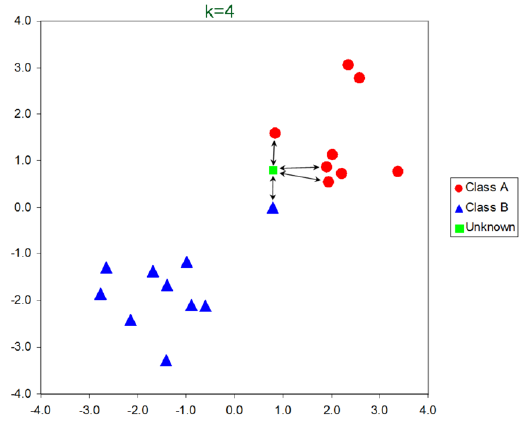
\includegraphics[scale=0.36]{img/knn.png}
	\caption{representação visual de 19 vetores rotulados com classe A e B e uma
	classe desconhecida. O vetor com classe desconhecida é portanto, rotulado
	com seus 4 (k=4) vizinhos mais próximos de acordo com a distância euclidiana
	entre eles.}
	\label{fig:fig1}
\end{figure}

Um conjunto de treino X consiste em n pares de vetores e rótulos, dispersos em
um espaço de classes. Dado um novo par (x; $\theta$), onde apenas a medida x é
observável, o valor de $\theta$	é estimado pela utilização dos dados contidos
no conjunto X com os vetores e rótulos já conhecidos (supervisionado). Um vetor
x' é um vizinho mais próximo de x, se segundo a Equação:

$d(x_{n}', x) = min(x_i, x) i = 1, 2, ...,n$

A distância mínima entre um vetor vizinho e o vetor testado são iguais ao 
conjunto de distâncias mínimas entre os outros vetores e o vetor testado. 
Normalmente, o ``voto'' do vizinho possui um peso, de acordo com a distância do
vetor testado e seus ``k'' vizinhos mais próximos. Assim, $\theta$ é estimado 
com o rótulo desses ``k'' vizinhos mais próximos,como mostra a 
Figura~\ref{fig:fig1}.

